\documentclass[9pt, aspectratio=169]{beamer}

% --- Theme Selection ---
\usetheme{metropolis} 

% --- Color Customization ---
\definecolor{DeepPurple}{HTML}{4B0082}
\definecolor{RoyalBlue}{HTML}{002366}
\definecolor{SoftPurple}{HTML}{9370DB}
\definecolor{CyanBlue}{HTML}{00BFFF}

\setbeamercolor{palette primary}{bg=RoyalBlue, fg=white}
\setbeamercolor{palette secondary}{bg=DeepPurple, fg=white}
\setbeamercolor{title}{fg=DeepPurple}
\setbeamercolor{progress bar}{fg=CyanBlue, bg=SoftPurple}
\setbeamercolor{block title}{bg=RoyalBlue, fg=white}

% --- Packages ---
\usepackage[utf8]{inputenc}
\usepackage{booktabs}
\usepackage{amsmath}
\usepackage{graphicx}
\usepackage{tikz}

% --- Presentation Info ---
\title{The Identification of Exoplanets using Physics-Aware Machine Learning}
\subtitle{Phase II: Model Implementation and Results}
\author{Esraaj Sarkar Gupta \and Suyash Prakash \and Anirudh Puri}
\date{May 2026}
\institute{Machine Learning and Pattern Recognition | Plaksha University}

\begin{document}

% ==============================
% SLIDE 0: Title Slide
% ==============================
\maketitle

% ==============================
% SLIDE 1: Project Scope & Thesis
% ==============================
\begin{frame}{The Project: Beyond Black-Box Models}
    \textbf{Core Objective:} \\
    We aim to identify and validate exoplanets by integrating fundamental orbital mechanics into classical machine learning architectures. 
    
    \vspace{1em}
    \textbf{Our Thesis:} \\
    Physics-Informed Machine Learning (PIML) provides superior interpretability, robustness, and performance over purely data-driven models. By engineering physical boundaries, we dramatically reduce sample complexity.
    
    \vspace{1em}
    \begin{quote}
        ``Early results show that relatively simple ML techniques paired with well-engineered features often perform comparable to much more complex ML models... critical for establishing credibility.'' \footnotemark
    \end{quote}
    
    \footnotetext[1]{Ford, E. B. (2025). Enhancing Exoplanet Surveys via Physics-informed Machine Learning. \textit{Proc. of the IAU}.}
\end{frame}

% ==============================
% SLIDE 2: Datasets
% ==============================
\begin{frame}{Mission Overview \& Datasets}
    Our analysis leverages data from three distinct phases of space-based transit photometry.\footnotemark
    
    \vspace{1em}
    \begin{columns}[T]
        \begin{column}{0.31\textwidth}
            \textbf{\textcolor{DeepPurple}{Kepler DR25 (KOI)}}\\
            \textit{The Gold Standard}\\
            Four years of continuous monitoring in a fixed field. Provided the highly stable, complete cases used to train our physical anchors.
        \end{column}
        
        \begin{column}{0.31\textwidth}
            \textbf{\textcolor{DeepPurple}{K2 Mission}}\\
            \textit{Kepler Extended}\\
            Born from the mechanical failure of Kepler’s reaction wheels. Surveyed the ecliptic plane using solar radiation pressure for stability.
        \end{column}
        
        \begin{column}{0.31\textwidth}
            \textbf{\textcolor{DeepPurple}{TESS}}\\
            \textit{Current Survey}\\
            An all-sky scanning mission focusing on stars 30-100x brighter than those in the Kepler field. Exhibits high sparsity.
        \end{column}
    \end{columns}
    \footnotetext[2]{Data sourced from the NASA Exoplanet Archive: \url{https://exoplanetarchive.ipac.caltech.edu/}}
\end{frame}

% ==============================
% SLIDE 3: Data Preprocessing Timeline
% ==============================
\begin{frame}{Data Preprocessing Pipeline}
    \begin{center}
    \resizebox{\textwidth}{!}{
    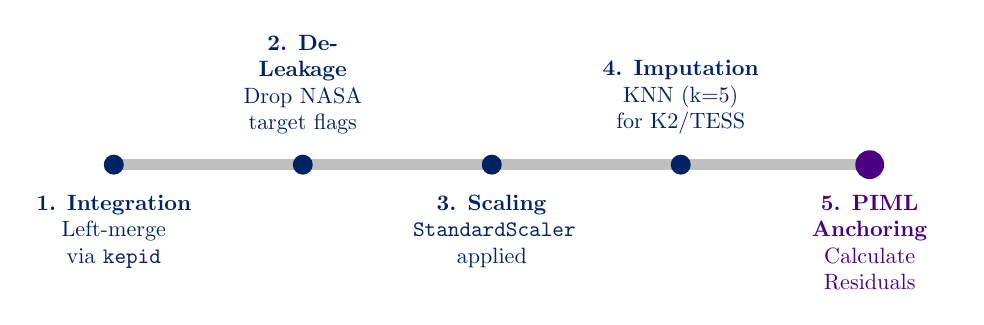
\begin{tikzpicture}[node distance=2.5cm, auto, thick, scale=0.8, every node/.style={transform shape}]
        % Timeline line
        \draw[lightgray, line width=4pt] (0,0) -- (12,0);
        
        % Nodes
        \filldraw[RoyalBlue] (0,0) circle (4pt) node[align=center, below=10pt, text width=2.5cm] {\textbf{1. Integration}\\Left-merge via \texttt{kepid}};
        \filldraw[RoyalBlue] (3,0) circle (4pt) node[align=center, above=10pt, text width=2.5cm] {\textbf{2. De-Leakage}\\Drop NASA target flags};
        \filldraw[RoyalBlue] (6,0) circle (4pt) node[align=center, below=10pt, text width=2.5cm] {\textbf{3. Scaling}\\\texttt{StandardScaler} applied};
        \filldraw[RoyalBlue] (9,0) circle (4pt) node[align=center, above=10pt, text width=2.5cm] {\textbf{4. Imputation}\\KNN (k=5) for K2/TESS};
        \filldraw[DeepPurple] (12,0) circle (6pt) node[align=center, below=10pt, text width=2.5cm] {\textbf{5. PIML Anchoring}\\Calculate Residuals};
    \end{tikzpicture}
    }
    \end{center}
    
    \vspace{2em}
    \textbf{Handling Sparsity:} Kepler data was robust enough for complete-case analysis. However, TESS and K2 exhibited severe observational gaps (nearly every row contained a \texttt{NaN}). Distance-weighted KNN imputation was vital to preserve physical covariance structures before feature engineering.
\end{frame}

% ==============================
% SLIDE 4: Derived Features & Anchors
% ==============================
\begin{frame}{Physics-Informed Feature Engineering}
    To constrain our machine learning models, we explicitly calculate the residuals ($\Delta$) between the telescope's observations and theoretical orbital mechanics.
    
    \vspace{0.5em}
    
    \begin{itemize}
        \item \textbf{1. Transit Depth Consistency} ($\Delta\delta$)
        \[
            \delta_{\text{theo}} = \left(\frac{R_p}{R_*}\right)^2 \quad \Longrightarrow \quad \Delta\delta = |\delta_{\text{obs}} - \delta_{\text{theo}}|
        \]
        \vspace{0.2em}
        
        \item \textbf{2. Transit Duration Consistency} ($\Delta T$)
        \[
            T_{\text{theo}} = \frac{P}{\pi} \arcsin\left(\frac{R_* \sqrt{1-b^2}}{a}\right) \quad \Longrightarrow \quad \Delta T = |T_{\text{obs}} - T_{\text{theo}}|
        \]
        \vspace{0.2em}
        
        \item \textbf{3. Impact Parameter Consistency} ($\Delta b^2$)
        \[
            b^2_{\text{theo}} = \left(1 - \sqrt{\delta}\right)^2 - \left(\frac{a}{R_*} \sin\left(\frac{T \pi}{P}\right)\right)^2 \quad \Longrightarrow \quad \Delta b^2 = |b^2_{\text{obs}} - b^2_{\text{theo}}|
        \]
    \end{itemize}
\end{frame}

% ==============================
% SLIDE 5: Validation Graphs
% ==============================
\begin{frame}{Validating Theoretical Anchors}
    \textbf{Separation of Classes via Physical Residuals:} 
    Before passing data to the model, we verified that our engineered physics residuals naturally isolate False Positives (red) from Confirmed Exoplanets (green).
    
    \vspace{1em}
    \begin{figure}
        \centering
        % Ensure these images are in the same folder as your .tex file
        \includegraphics[width=0.32\textwidth]{depth_residual.png}
        \hfill
        \includegraphics[width=0.32\textwidth]{duration_residual.png}
        \hfill
        \includegraphics[width=0.32\textwidth]{b_residual.png}
        \vspace{-0.5em}
        \caption{Distributions of residuals for Transit Depth, Duration, and Impact Parameter ($b^2$). Confirmed planets tightly hug zero (theoretical agreement), while false positives cascade outward.}
    \end{figure}
\end{frame}

% ==============================
% SLIDE 6: Model Selection
% ==============================
\begin{frame}{Model Architecture Selection: SVM vs. RFC}
    To capture complex, non-linear relationships without the overhead of deep learning, we initially selected Support Vector Classifiers (SVC) and Random Forest Classifiers (RFC) as our core baselines.
    
    \vspace{-0.5em}
    \begin{figure}
        \centering
        \includegraphics[width=0.48\textwidth]{svc_vs_rfc_acc.png}
        \hfill
        \includegraphics[width=0.48\textwidth]{rfc_vs_svc_prauc.png}
    \end{figure}
    
    \vspace{-1em}
    \center
    \textbf{RFC significantly outperformed SVM across all folds.}
\end{frame}

% ==============================
% SLIDE 7: Ablation Study
% ==============================
\begin{frame}{Ablation Study: Data-Driven vs. Physics-Informed (RFC)}
    We conducted a head-to-head ablation study comparing a purely Data-Driven approach vs. our Best PIML framework.
    
    \vspace{-0.5em}
    \begin{figure}
        \centering
        \includegraphics[width=0.48\textwidth]{ablation_acc.png}
        \hfill
        \includegraphics[width=0.48\textwidth]{pr_auc_ablation.png}
    \end{figure}

\end{frame}

% ==============================
% SLIDE 7.5: Ablation Insight (The K2 Noise Problem)
% ==============================
\begin{frame}{Ablation Insight: The Impact of Non-Gaussian Noise}
    \textbf{The K2 Anomaly Explained:} \\
    Why did our purely data-driven model outperform the physics-anchored framework specifically on the K2 dataset?
    
    \vspace{1em}
    \begin{table}[]
        \centering
        \footnotesize
        \begin{tabular}{l cc}
            \toprule
            \textbf{K2 Dataset Performance} ($k=10$ Cross-Val) & Accuracy & PR-AUC \\
            \midrule
            \textbf{Data-Driven (Ablation Set)} & \textbf{0.8380} & \textbf{0.9375} \\
            \textbf{Physics-Informed (Features 4)} & 0.7879 & 0.8855 \\
            \bottomrule
        \end{tabular}
    \end{table}
    
    \vspace{0.5em}
    Recent literature confirms that Physics-Informed models degrade significantly under non-Gaussian noise.\footnotemark \ Rigid physical equations force the model to fit to flawed theoretical assumptions, whereas unconstrained data-driven models adaptively learn and bypass the noise distribution.

    \footnotetext{Pilar, P., \& Wahlström, N. (2023). Physics-informed neural networks with unknown measurement noise. \textit{NeurIPS 2023 Workshop on Machine Learning and the Physical Sciences}.}
\end{frame}

% ==============================
% SLIDE 8: HistGB & Imputation Validation
% ==============================
\begin{frame}{Handling Sparsity: HistGB vs. KNN Imputation}
    \textbf{What is HistGradientBoosting (HistGB)?} \\
    It is a highly efficient, histogram-based tree architecture. Crucially, unlike Random Forests, HistGB \footnotemark \ \textbf{natively handles missing values (NaNs)} by learning during training which child node the missing data should be routed to.
    
    \vspace{0.5em}
    
    \vspace{-0.5em}
    \begin{figure}
        \centering
        \includegraphics[width=0.48\textwidth]{k2_imputed.png}
        \hfill
        \includegraphics[width=0.48\textwidth]{tess_imputed.png}
    \end{figure}
    
    \footnotetext{Ke, G., et al. (2017). LightGBM: A Highly Efficient Gradient Boosting Decision Tree. \textit{NIPS 2017}. (The basis for Scikit-Learn's HistGradientBoosting).}
\end{frame}

% ==============================
% SLIDE 9: Deep Learning Challenger: TabNet
% ==============================
\begin{frame}{Comparisons with Deep Learning: TabNet}
    \textbf{What is TabNet?} \\
    Developed by researchers at Google Cloud AI, TabNet\footnotemark \ is a deep learning architecture designed specifically for tabular data. It uses a sequential attention mechanism to choose which features to reason from at each decision step.

    \begin{figure}
        \centering
        % Displaying your TabNet comparison image
        \includegraphics[width=\textwidth]{tabnet_vs_best.png}
        \vspace{-0.5em}
        %\caption{Comparison of TabNet performance against our best-performing RFC and HistGB models across datasets.}
    \end{figure}

    \footnotetext{Arik, S. O., \& Pfister, T. (2021). TabNet: Attentive Interpretable Tabular Learning. \textit{AAAI Conference on Artificial Intelligence}.}
\end{frame}


% ==============================
% SLIDE 10: Model Explainability
% ==============================
\begin{frame}{Model Explainability: Opening the "Black Box"}
    A core advantage of Classical ML over Deep Learning is the retention of \textbf{Explainability}. Using Mean Gini Importance, we can quantify exactly which features drive the model's decisions.

    \vspace{0.5em}
    \begin{figure}
        \centering
        % Side-by-side-by-side layout
        \begin{columns}
            \begin{column}{0.33\textwidth}
                \centering
                \includegraphics[width=\linewidth]{KOI_feature_importance.png}
                \caption{\small \textbf{Kepler (KOI)}}
            \end{column}
            \begin{column}{0.33\textwidth}
                \centering
                \includegraphics[width=\linewidth]{TESS_feature_importance.png}
                \caption{\small \textbf{TESS}}
            \end{column}
            \begin{column}{0.33\textwidth}
                \centering
                \includegraphics[width=\linewidth]{K2_feature_importance.png}
                \caption{\small \textbf{K2}}
            \end{column}
        \end{columns}
    \end{figure}

    \vspace{-0.5em}
\end{frame}

% ==============================
% SLIDE 11: Conclusion & Q&A
% ==============================
\begin{frame}[standout]
    Questions?
    
    \vspace{2em}
    \begin{center}
        \Huge Thank You!
    \end{center}
    \vspace{2em}
    
    \normalsize
    \textbf{Esraaj Sarkar Gupta $\bullet$ Suyash Prakash $\bullet$ Anirudh Puri} \\
    Machine Learning and Pattern Recognition | Plaksha University
\end{frame}

\end{document}